\section{Application: Perspective rendering}

As an application of linear transformations, we consider the problem
of perspective rendering. Imagine some object has been described by
coordinates in 3-dimensional space, and we wish to make an image of
the object as it would be seen by a human eye or by a camera. The
process of computing such an image is known as \textbf{rendering}%
\index{rendering}.

Conceptually, the rendering process makes use of a \textbf{camera}%
\index{camera}, which we will assume is located at the origin of a
3-dimensional coordinate system called the \textbf{camera coordinate
  system}%
\index{camera coordinates}%
\index{coordinate system!camera coordinates}, and an \textbf{image
  plane}%
\index{image plane}%
\index{plane!image plane}, which we will assume is the plane $z=1$ in
camera coordinates. The 3-dimensional space also contains one or more
objects that we wish to render. We can consider the object to be
described by a set of points. For each point $\vect{p}$ on the object,
draw a straight line from $\vect{p}$ to the camera, and let
$\vect{p}'$ be the point where this line intersects the image
plane. The point $\vect{p}$ of the object is rendered as the point
$\vect{p}'$ in the image. This process is illustrated in the following
figure:
\begin{equation*}
  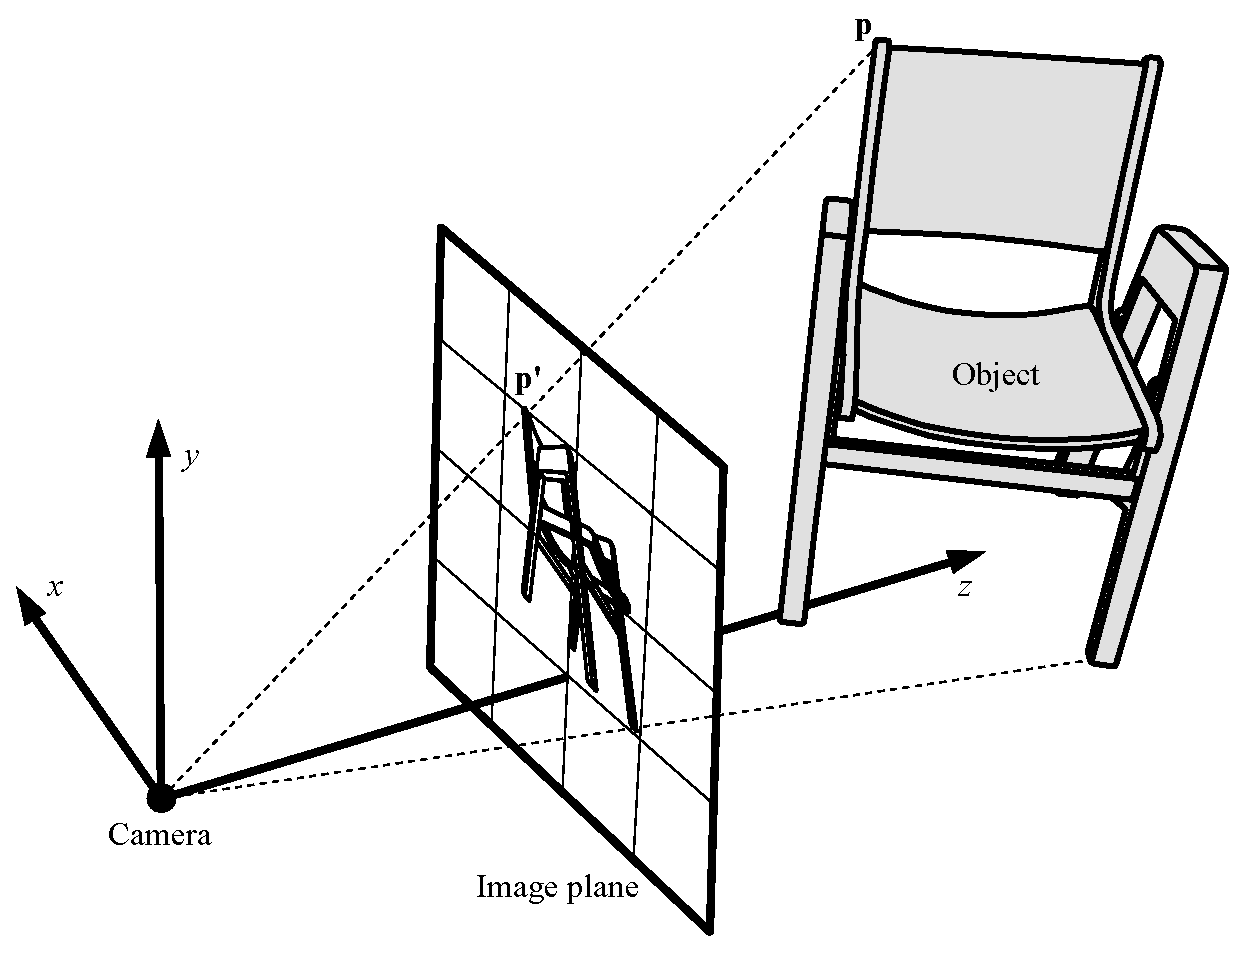
\includegraphics[width=0.90\textwidth]{figures/perspective-chair}
\end{equation*}

% ----------------------------------------------------------------------
\subsection*{Object coordinates}

It is convenient to describe each object in its own coordinate system,
called the \textbf{object coordinate system}%
\index{object coordinates}%
\index{coordinate system!object coordinates}. To illustrate this
concept, we will consider a cube of side length 2, centered at the
origin. The 8 corners of this cube have the following coordinates in
the object coordinate system:
\begin{equation*}
  \begin{mymatrix}{r}  1 \\  1 \\  1 \end{mymatrix},~
  \begin{mymatrix}{r}  1 \\  1 \\ -1 \end{mymatrix},~
  \begin{mymatrix}{r}  1 \\ -1 \\  1 \end{mymatrix},~
  \begin{mymatrix}{r}  1 \\ -1 \\ -1 \end{mymatrix},~
  \begin{mymatrix}{r} -1 \\  1 \\  1 \end{mymatrix},~
  \begin{mymatrix}{r} -1 \\  1 \\ -1 \end{mymatrix},~
  \begin{mymatrix}{r} -1 \\ -1 \\  1 \end{mymatrix},~
  \begin{mymatrix}{r} -1 \\ -1 \\ -1 \end{mymatrix}.
\end{equation*}
For later reference, let us call this the \textbf{standard cube}%
\index{standard cube}. The following picture shows the standard cube
within its object coordinate system:
\begin{equation*}
  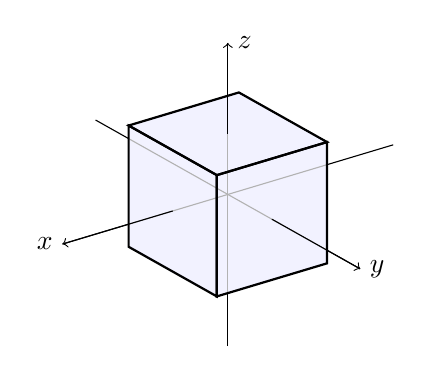
\begin{tikzpicture}[x={(0.8cm,-0.45cm)},y={(1cm,0.3cm)},z={(0cm,1.1cm)},scale=0.7]
    \draw[->] (-3,0,0) -- (3,0,0) node[right]{$y$};
    \draw[->] (0,3,0) -- (0,-3,0) node[left]{$x$};
    \draw[->] (0,0,-2.5) -- (0,0,2.5) node[right]{$z$};
    \begin{scope}
      \clip (1,1,1) -- (1,1,-1) -- (1,-1,-1) -- (-1,-1,-1)
      -- (-1,-1,1) -- (-1,1,1) -- cycle;
      \fill[blue!5] (1,1,1) -- (1,1,-1) -- (1,-1,-1) -- (-1,-1,-1)
      -- (-1,-1,1) -- (-1,1,1) -- cycle;
      \draw[black!30,->] (-3,0,0) -- (3,0,0);
      \draw[black!30,->] (0,-3,0) -- (0,3,0);
      \draw[black!30,->] (0,0,-2.5) -- (0,0,2.5);
    \end{scope}
    \draw[thick] ( 1, 1, 1) -- ( 1, 1,-1) -- ( 1,-1,-1) -- ( 1,-1, 1) -- cycle;
    \draw[thick] ( 1,-1, 1) -- (-1,-1, 1) -- (-1,-1,-1) -- ( 1,-1,-1) -- cycle;
    \draw[thick] ( 1, 1, 1) -- ( 1,-1, 1) -- (-1,-1, 1) -- (-1, 1, 1) -- cycle;
    \draw (1,0,0) -- (3,0,0);
    \draw (0,-3,0) -- (0,-1,0);
    \draw (0,0,1) -- (0,0,2.5);
  \end{tikzpicture}
\end{equation*}

% ----------------------------------------------------------------------
\subsection*{Conversion to camera coordinates}

Before we render an object, we need to place it in some appropriate
location relative to the camera. We do this by specifying four vectors
$\vect{q}$, $\vect{a}_x$, $\vect{a}_y$, and $\vect{a}_z$ in
$\R^3$. Here, $\vect{q}$ is the origin of the object coordinate
system, relative to the camera coordinate system. The vectors
$\vect{a}_x$, $\vect{a}_y$, and $\vect{a}_z$ are the axes of the
object coordinate system, relative to the camera coordinate system, as
shown in the following illustration:
\begin{equation*}
  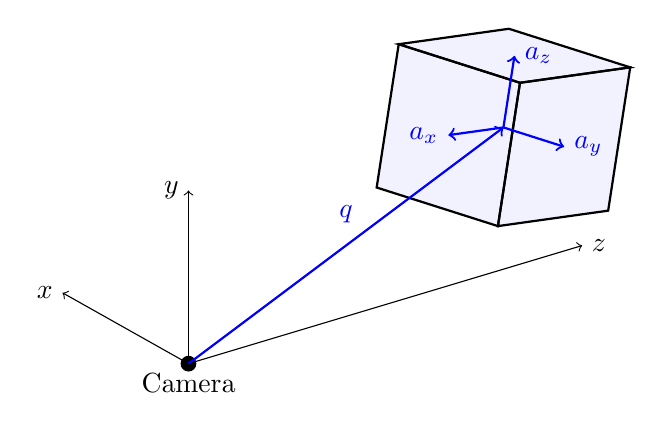
\begin{tikzpicture}
    \fill (0,0) circle (0.1) node[below] {Camera};
    \begin{scope}[x={(-0.8cm,0.45cm)},z={(1cm,0.3cm)},y={(0cm,1.1cm)}]
      \draw[->] (0,0,0) -- (2,0,0) node[left]{$x$};
      \draw[->] (0,0,0) -- (0,2,0) node[left]{$y$};
      \draw[->] (0,0,0) -- (0,0,5) node[right]{$z$};
    \end{scope}
    \begin{scope}[shift={(4,3)}]
      \begin{scope}[x={(-1cm,-0.14cm)},y={(1.1cm,-0.35cm)},z={(0.2cm,1.3cm)},scale=0.7]
        \begin{scope}
          \clip (1,-1,1) -- (1,-1,-1) -- (1,1,-1) -- (-1,1,-1)
          -- (-1,1,1) -- (-1,-1,1) -- cycle;
          \fill[blue!5] (1,-1,1) -- (1,-1,-1) -- (1,1,-1) -- (-1,1,-1)
          -- (-1,1,1) -- (-1,-1,1) -- cycle;
        \end{scope}
        \draw[thick] ( 1, 1, 1) -- ( 1, 1,-1) -- ( 1,-1,-1) -- ( 1,-1, 1) -- cycle;
        \draw[thick] ( 1, 1, 1) -- (-1, 1, 1) -- (-1, 1,-1) -- ( 1, 1,-1) -- cycle;
        \draw[thick] ( 1, 1, 1) -- ( 1,-1, 1) -- (-1,-1, 1) -- (-1, 1, 1) -- cycle;
        \draw[thick,blue,->] (0,0,0) -- (1,0,0) node[left]{$\vect{a}_x$};
        \draw[thick,blue,->] (0,0,0) -- (0,1,0) node[right]{$\vect{a}_y$};
        \draw[thick,blue,->] (0,0,0) -- (0,0,1) node[right]{$\vect{a}_z$};
      \end{scope}
    \end{scope}
    \draw[thick,blue,->] (0,0) -- node[above=1ex]{$\vect{q}$}(4,3);
  \end{tikzpicture}
\end{equation*}
Thus, given a point with object coordinates
$\vect{v}=\begin{mymatrix}{c}x\\y\\z\end{mymatrix}$, we can find its
camera coordinates
$\vect{p} = \begin{mymatrix}{c} p_x \\ p_y \\ p_z \end{mymatrix}$ by
the following formula:
\begin{equation*}
  \vect{p} = \vect{q} + x\vect{a}_x + y\vect{a}_y + z\vect{a}_z.
\end{equation*}
If we write $A$ for the $3\times 3$-matrix whose columns are $\vect{a}_x$,
$\vect{a}_y$, and $\vect{a}_z$, we can also write this formula more succinctly as
\begin{equation*}
  \vect{p} = \vect{q} + A\vect{v}.
\end{equation*}

\begin{example}{Converting object coordinates to camera coordinates}{object-to-camera}
  Let
  \begin{equation*}
    \vect{q} = \begin{mymatrix}{c} 0 \\ 2 \\ 10 \end{mymatrix},\quad
    A = \begin{mymatrix}{ccc}
      0.8 & 0.6 & 0 \\
      0 & 0 & 1 \\
      0.6 & -0.8 & 0 \\
    \end{mymatrix}.
  \end{equation*}
  Convert each of the 8 corners of the standard cube from object
  coordinates to camera coordinates.
\end{example}

\begin{solution}
  Let $\vect{v}_1,\ldots,\vect{v}_8$ be the object coordinates of the
  8 corners of the cube:
  \begin{equation*}
    \begin{mymatrix}{r}  1 \\  1 \\  1 \end{mymatrix},~
    \begin{mymatrix}{r}  1 \\  1 \\ -1 \end{mymatrix},~
    \begin{mymatrix}{r}  1 \\ -1 \\  1 \end{mymatrix},~
    \begin{mymatrix}{r}  1 \\ -1 \\ -1 \end{mymatrix},~
    \begin{mymatrix}{r} -1 \\  1 \\  1 \end{mymatrix},~
    \begin{mymatrix}{r} -1 \\  1 \\ -1 \end{mymatrix},~
    \begin{mymatrix}{r} -1 \\ -1 \\  1 \end{mymatrix},~
    \begin{mymatrix}{r} -1 \\ -1 \\ -1 \end{mymatrix}.
  \end{equation*}
  We convert each of them to camera coordinates using the formula
  $\vect{p}_i = \vect{q} + A\vect{v}_i$:
  \begin{eqnarray*}
    \vect{p}_1 &=&
    \begin{mymatrix}{c} 0 \\ 2 \\ 10 \end{mymatrix}
    + \begin{mymatrix}{ccc}
      0.8 & 0.6 & 0 \\
      0 & 0 & 1 \\
      0.6 & -0.8 & 0 \\
    \end{mymatrix}
    \begin{mymatrix}{r}  1 \\  1 \\  1 \end{mymatrix}
    ~=~
    \begin{mymatrix}{r}  1.4 \\  3.0 \\ 9.8 \end{mymatrix}, \\
    \vect{p}_2 &=&
    \begin{mymatrix}{c} 0 \\ 2 \\ 10 \end{mymatrix}
    + \begin{mymatrix}{ccc}
      0.8 & 0.6 & 0 \\
      0 & 0 & 1 \\
      0.6 & -0.8 & 0 \\
    \end{mymatrix}
    \begin{mymatrix}{r}  1 \\  1 \\ -1 \end{mymatrix}
    ~=~
    \begin{mymatrix}{r}  1.4 \\ 1.0 \\ 9.8 \end{mymatrix}, \\
    \vect{p}_3 &=&
    \begin{mymatrix}{c} 0 \\ 2 \\ 10 \end{mymatrix}
    + \begin{mymatrix}{ccc}
      0.8 & 0.6 & 0 \\
      0 & 0 & 1 \\
      0.6 & -0.8 & 0 \\
    \end{mymatrix}
    \begin{mymatrix}{r}  1 \\ -1 \\ 1 \end{mymatrix}
    ~=~
    \begin{mymatrix}{r}  0.2 \\ 3.0 \\ 11.4 \end{mymatrix}, \\
  \end{eqnarray*}
  and so on. Continuing in the same fashion, we find
  $\vect{p}_1,\ldots,\vect{p}_8$:
  \begin{equation}\label{eqn:object-to-camera}
    \begin{mymatrix}{r}  1.4 \\ 3.0 \\ 9.8 \end{mymatrix},
    \begin{mymatrix}{r}  1.4 \\ 1.0 \\ 9.8 \end{mymatrix},
    \begin{mymatrix}{r}  0.2 \\ 3.0 \\ 11.4 \end{mymatrix},
    \begin{mymatrix}{r}  0.2 \\ 1.0 \\ 11.4 \end{mymatrix},
    \begin{mymatrix}{r} -0.2 \\ 3.0 \\ 8.6 \end{mymatrix},
    \begin{mymatrix}{r} -0.2 \\ 1.0 \\ 8.6 \end{mymatrix},
    \begin{mymatrix}{r} -1.4 \\ 3.0 \\ 10.2 \end{mymatrix},
    \begin{mymatrix}{r} -1.4 \\ 1.0 \\ 10.2 \end{mymatrix}.
  \end{equation}
\end{solution}

We can also write $f:\R^3 \to \R^3$ for the function that converts
object coordinates to camera coordinates, i.e.,
\begin{equation*}
  f(\vect{v}) = \vect{q} + A\vect{v}.
\end{equation*}
We note that this is not a linear function, because
$f(\vect{0})\neq \vect{0}$. The function $f$ is called an
\textbf{affine function}%
\index{function!affine}%
\index{affine function}, which means that it is a linear function
$\vect{v}\mapsto A\vect{v}$ followed by a translation
$\vect{v}\mapsto \vect{q}+\vect{v}$.

% ----------------------------------------------------------------------
\subsection*{Rendering}

Once we know the camera coordinates
$\vect{p}=\begin{mymatrix}{c} p_x \\ p_y \\ p_z \end{mymatrix}$ of a point,
we need to render the point, i.e., find its coordinates in the image plane.
\begin{equation*}
  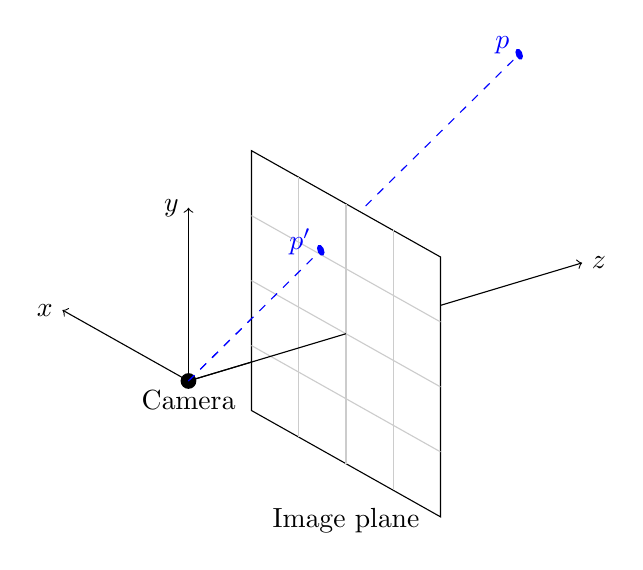
\begin{tikzpicture}
    \fill (0,0) circle (0.1) node[below] {Camera};
    \begin{scope}[x={(-0.8cm,0.45cm)},z={(1cm,0.3cm)},y={(0cm,1.1cm)}]
      \draw[->] (0,0,0) -- (2,0,0) node[left]{$x$};
      \draw[->] (0,0,0) -- (0,2,0) node[left]{$y$};
      \draw[->] (0,0,0) -- (0,0,5) node[right]{$z$};
      \draw[dashed,blue] (0,0,0) -- (1,2,5);
      \draw[fill=white] (-1.5,-1.5,2) -- (-1.5,1.5,2) -- (1.5,1.5,2) -- (1.5,-1.5,2) -- cycle;
      \draw[thin,black!20] (-1.5,-0.75,2) -- (1.5,-0.75,2);
      \draw[thin,black!20] (-1.5,0,2) -- (1.5,0,2);
      \draw[thin,black!20] (-1.5,0.75,2) -- (1.5,0.75,2);
      \draw[thin,black!20] (-0.75,-1.5,2) -- (-0.75,1.5,2);
      \draw[thin,black!20] (0,-1.5,2) -- (0,1.5,2);
      \draw[thin,black!20] (0.75,-1.5,2) -- (0.75,1.5,2);
      \fill[blue] (1,2,5) circle (0.06) +(0,0.1,0) node[left] {$\vect{p}$};
      \fill[blue] (0.4,0.8,2) circle (0.06) +(0,0.1,0) node[left] {$\vect{p}'$};
      \draw (0,0,0) -- (0,0,2);
      \draw[dashed,blue] (0,0,0) -- (0.4,0.8,2);
      \path (0,-1.9,2) node[below] {Image plane};
    \end{scope}
  \end{tikzpicture}
\end{equation*}
Since the camera is located at the origin, the line that passes
through the camera and the point $\vect{p}$ has the parametric equation
\begin{equation*}
  \vect{r} = t\vect{p} = \begin{mymatrix}{c} tp_x \\ tp_y \\ tp_z \end{mymatrix}.
\end{equation*}
Since the image plane is the plane $z=1$, we must set $t$ such that
$tp_z = 1$, i.e., $t=\frac{1}{p_z}$. Therefore, the coordinates of the
rendered point are
\begin{equation*}
  \vect{p}' = \frac{1}{p_z}\vect{p} =
  \begin{mymatrix}{c} p_x/p_z \\ p_y/p_z \\ 1 \end{mymatrix}.
\end{equation*}
Finally, since the image plane is $2$-dimensional, we can forget the
now useless $z$-coordinate, and render the point at the coordinates
$\begin{mymatrix}{c} p_x/p_z \\ p_y/p_z \end{mymatrix}$ in the
$2$-dimensional image plane.

\begin{example}{Rendering}{rendering}
  Render the cube from Example~\ref{exa:object-to-camera}.
\end{example}

\begin{solution}
  We must apply the rendering function
  \begin{equation*}
    g\paren{\begin{mymatrix}{c} p_x \\ p_y \\ p_z \end{mymatrix}}
    = \begin{mymatrix}{c} p_x/p_z \\ p_y/p_z \end{mymatrix}
  \end{equation*}
  to each of the corners of the cube from
  {\eqref{eqn:object-to-camera}}.
  We have
  \begin{eqnarray*}
    g\paren{\begin{mymatrix}{r}  1.4 \\ 3.0 \\ 9.8 \end{mymatrix}}
    &=& \begin{mymatrix}{r} 1.4/9.8 \\ 3.0/9.8 \end{mymatrix}
    ~=~ \begin{mymatrix}{r} 0.143 \\ 0.306 \end{mymatrix}, \\
    g\paren{\begin{mymatrix}{r}  1.4 \\ 1.0 \\ 9.8 \end{mymatrix}}
    &=& \begin{mymatrix}{r} 1.4/9.8 \\ 1.0/9.8 \end{mymatrix}
    ~=~ \begin{mymatrix}{r} 0.143 \\ 0.102 \end{mymatrix}, \\
    g\paren{\begin{mymatrix}{r}  0.2 \\ 3.0 \\ 11.4 \end{mymatrix}}
    &=& \begin{mymatrix}{r} 0.2/11.4 \\ 3.0/11.4 \end{mymatrix}
    ~=~ \begin{mymatrix}{r} 0.018 \\ 0.263 \end{mymatrix}, \\
  \end{eqnarray*}
  and so on. The 8 rendered points are:
  \begin{equation*}
    \begin{mymatrix}{r} 0.143 \\ 0.306 \end{mymatrix},~
    \begin{mymatrix}{r} 0.143 \\ 0.102 \end{mymatrix},~
    \begin{mymatrix}{r} 0.018 \\ 0.263 \end{mymatrix},~
    \begin{mymatrix}{r} 0.018 \\ 0.088 \end{mymatrix},~
    \begin{mymatrix}{r} -0.023 \\ 0.349 \end{mymatrix},~
    \begin{mymatrix}{r} -0.023 \\ 0.116 \end{mymatrix},~
    \begin{mymatrix}{r} -0.137 \\ 0.294 \end{mymatrix},~
    \begin{mymatrix}{r} -0.137 \\ 0.098 \end{mymatrix}.
  \end{equation*}
  Drawing these in the 2-dimensional image plane, we get the following
  picture:
  \begin{equation*}
    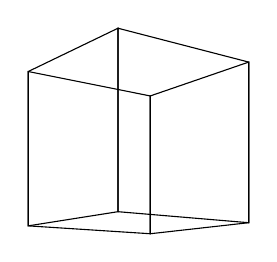
\begin{tikzpicture}[scale=10]
      \draw (0.143,0.306) -- (0.143,0.102) -- (0.018,0.088) -- (0.018,0.263) -- cycle;
      \draw (-0.023,0.349) -- (-0.023,0.116) -- (-0.137,0.098) -- (-0.137,0.294) -- cycle;
      \draw (0.143,0.306) -- (0.143,0.102) -- (-0.023,0.116) -- (-0.023,0.349) -- cycle;
      \draw (0.018,0.088) -- (0.018,0.263) -- (-0.137,0.294) -- (-0.137,0.098) -- cycle;
    \end{tikzpicture}
  \end{equation*}

\end{solution}
